\begin{figure}
    \centering
    \hspace*{49pt}
    %Chart: Mean scores (Dimension 3)
    \begin{tikzpicture}
        \begin{axis}[
            axis lines=left,
            axis x line=bottom,
            axis line style={draw=black,-},
            width  = .85\textwidth,
            height = .25\textheight,
            major x tick style = transparent,
            ybar=3.0*\pgflinewidth,
            bar width=6pt,
            xmajorgrids = true,
            ymajorgrids = false,
            yticklabels={},
            ylabel = {\scriptsize Mean score},
            symbolic x coords={Official documents,Professional letters,Press reviews,Academic prose,Religion,Popular lore,Press editorials,Biographies,Spontaneous speeches,Hobbies,Prepared speeches,Press reportage,Interviews,Humor,Science fiction,General fiction,Mystery fiction,Personal letters,Adventure fiction,Face-to-face conversations,Romantic fiction,Telephone conversations,Broadcasts},
            xtick = data,
            nodes near coords,
            every node near coord/.append style={/pgf/number format/fixed},
            every node near coord/.append style={font=\tiny},
            every node near coord/.append style={rotate=90,anchor=west},
            nodes near coords style={/pgf/number format/.cd,precision=1},
            every axis/.append style={label style={font=\footnotesize},tick label style={font=\footnotesize}},
            x tick label style={rotate=30,anchor=east,font=\tiny,xshift=5pt},
            scaled y ticks = false,
            enlarge y limits={abs=.2*\pgfplotbarwidth},
            enlarge x limits={abs=1.5*\pgfplotbarwidth},
            extra y ticks = 0,
            extra y tick labels={},
            extra y tick style={grid=major,major grid style={thick,densely dashed,draw=red}}
        ]
        \addplot[style={draw=black,fill=red!50,mark=none}]
            coordinates {
                (Official documents,7.3)
                (Professional letters,6.5)
                (Press reviews,4.3)
                (Academic prose,4.2)
                (Religion,3.7)
                (Popular lore,2.3)
                (Press editorials,1.9)
                (Biographies,1.7)
                (Spontaneous speeches,1.2)
                (Hobbies,0.3)
                (Prepared speeches,0.3)
                (Press reportage,-0.3)
                (Interviews,-0.4)
                (Humor,-0.8)
                (Science fiction,-1.4)
                (General fiction,-3.1)
                (Mystery fiction,-3.6)
                (Personal letters,-3.6)
                (Adventure fiction,-3.8)
                (Face-to-face conversations,-3.9)
                (Romantic fiction,-4.1)
                (Telephone conversations,-5.2)
                (Broadcasts,-9)
            };
        \end{axis}
    \end{tikzpicture}
    %Chart: Loadings (Dimension 3)
    \begin{tikzpicture}
        \begin{axis}[
            axis lines=left,
            axis x line=bottom,
            axis line style={draw=black,-},
            width  = .85\textwidth,
            height = .25\textheight,
            major x tick style = transparent,
            ybar=3.0*\pgflinewidth,
            bar width=6pt,
            xmajorgrids = true,
            ymajorgrids = false,
            yticklabels={},
            ylabel = {\scriptsize Loading},
            symbolic x coords={WH relative clauses on object positions,Pied piping constructions,WH relative clauses on subject positions,Nominalizations,Phrasal coordination,Adverbs,Place adverbials,Time adverbials},
            xtick = data,
            nodes near coords,
            every node near coord/.append style={/pgf/number format/fixed},
            every node near coord/.append style={font=\tiny},
            every node near coord/.append style={rotate=90,anchor=west},
            nodes near coords style={/pgf/number format/.cd,precision=1},
            every axis/.append style={label style={font=\footnotesize},tick label style={font=\footnotesize}},
            x tick label style={rotate=30,anchor=east,font=\tiny,xshift=5pt},
            scaled y ticks = false,
            enlarge y limits={abs=.2*\pgfplotbarwidth},
            enlarge x limits={abs=1.5*\pgfplotbarwidth},
            extra y ticks = 0,
            extra y tick labels={},
            extra y tick style={grid=major,major grid style={thick,densely dashed,draw=red}}
        ]
        \addplot[style={draw=black,fill=blue!25,mark=none}]
            coordinates {
                (WH relative clauses on object positions,0.63)
                (Pied piping constructions,0.61)
                (WH relative clauses on subject positions,0.45)
                (Nominalizations,0.36)
                (Phrasal coordination,0.36)
                (Adverbs,-0.46)
                (Place adverbials,-0.49)
                (Time adverbials,-0.60)
            };
        \end{axis}
    \end{tikzpicture}
    \caption{Dimensão 3 -- Referências Explícitas versus Referências Dependentes do Contexto \citep[Original em língua inglesa]{biberVariationSpeechWriting1988}}
    \label{fig:merged_dim3_biber_ptbr}
\end{figure}
